\begin{figure*}
	\begin{center}
		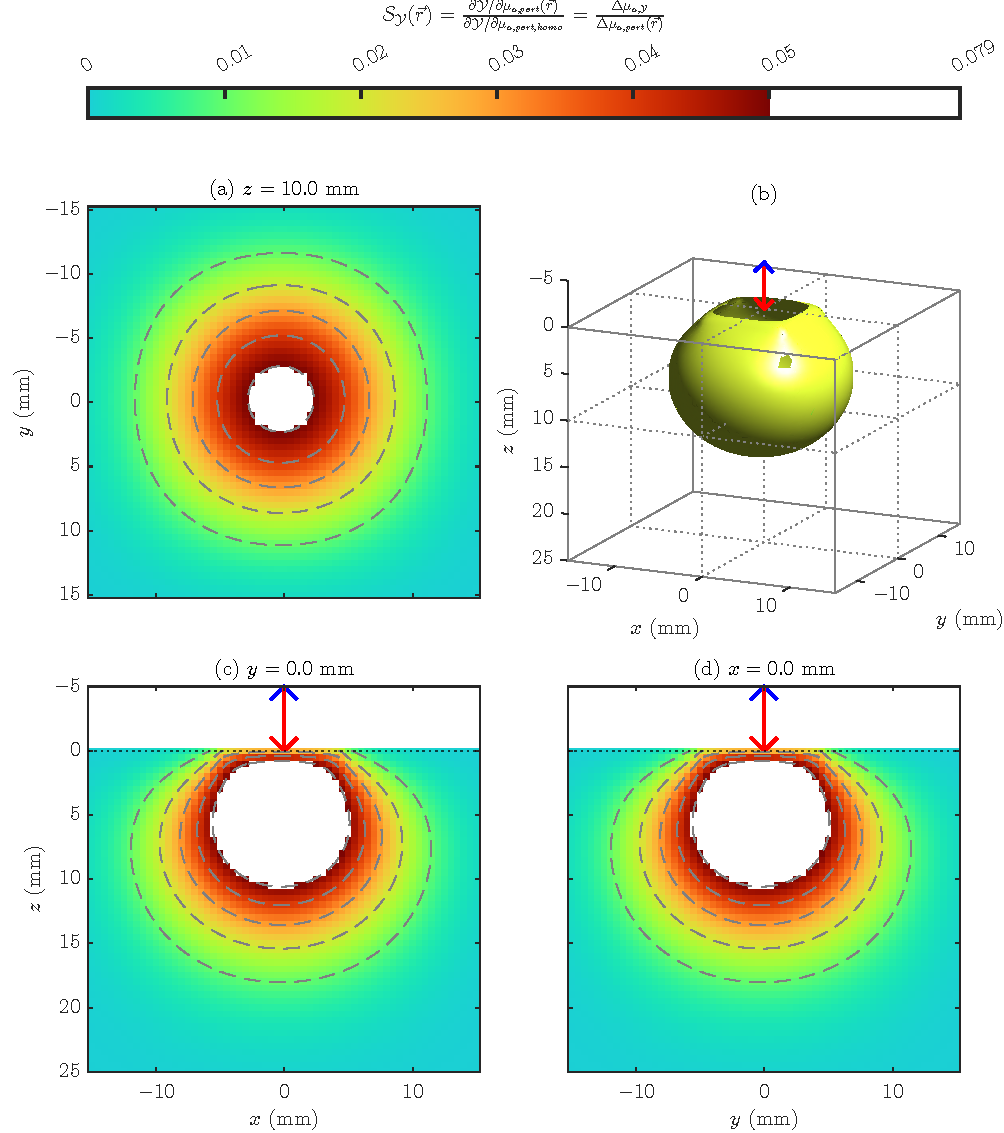
\includegraphics{\gitPath makeFigs/Figs/TD_SD_GI_3rd_rho0_MC_301.pdf}
	\end{center}
	\caption{Third angle projection of the \acrfull{sen} to a $\SI{10.0}{\milli\meter}\times\SI{10.0}{\milli\meter}\times\SI{2.0}{\milli\meter}$ perturbation scanned \SI{0.5}{\milli\meter} measured by \acrfull{TD} \acrfull{SD} gated \acrfull{I}. (a) $x$-$y$ plane sliced at $z=\SI{10.0}{\milli\meter}$. (b) Iso-surface sliced at $\as{S}=0.020$. (c) $x$-$z$ plane sliced at $y=\SI{0.0}{\milli\meter}$. (d) $y$-$z$ plane sliced at $x=\SI{0.0}{\milli\meter}$. Generated using \acrfull{MC}.\\ 
	\Acrfull{rho}: \SI{0.0}{\milli\meter}\\ 
	\Acrfull{n} inside: \num{1.333};\quad	\Acrfull{n} outside: \num{1.000}\\ 
	\Acrfull{musp}: \SI{1.10}{\per\milli\meter};\quad	\Acrfull{g}: \num{0.9}\\ 
	\Acrfull{mua}: \SI{0.011}{\per\milli\meter}\\ 
	\Acrfull{t} gate: [1500, 2000]~\si{\pico\second}\\ 
	Detector Numerical Aperature (NA): \num{0.5};\quad	Number of photons: \num{1000000000}\\ 
	}\label{fig:TD_SD_GI_3rd_rho0_MC}
\end{figure*}
